
\begin{figure}[H]
\centering
\includegraphics[page=8,width=0.4\textwidth]{\FCNCFigures/tthML/showFake/faketau/postfit/NOMINAL/reg1l1tau1b3j_os_vetobtagwp70_highmet/x1fit.pdf}
\put(-140, 92){\footnotesize{$t_h\tlhad$-3j}}
\includegraphics[page=8,width=0.4\textwidth]{\FCNCFigures/tthML/showFake/faketau/postfit/NOMINAL/reg1l1tau1b3j_os_vetobtagwp70_highmet/x2fit.pdf}
\put(-140, 92){\footnotesize{$t_h\tlhad$-3j}}\\
\includegraphics[page=6,width=0.4\textwidth]{\FCNCFigures/xTFW/showFake/NOMINAL/reg2mtau1b3jos_vetobtagwp70_highmet/x1fit.pdf}
\put(-140, 105){\footnotesize{$t_h\thadhad$-3j}}
\includegraphics[page=6,width=0.4\textwidth]{\FCNCFigures/xTFW/showFake/NOMINAL/reg2mtau1b3jos_vetobtagwp70_highmet/x2fit.pdf}
\put(-140, 105){\footnotesize{$t_h\thadhad$-3j}}
\caption{ The distributions of the momentum fraction carried by the visible decay products from the tau mother $E_{\nu,i}/E_{\tau,i},i=1,2$ in the $t_h\tlhad$-3j (top) and $\thadhad$ (bottom) channels in terms of tuH merged signal. The real tau contributions shown from ttbar and other MC including diboson, single top, and V+jets. Only statistical uncertainties are being shown. Underflow and overflow bins are included respectively in the first and last bins.}
\label{fig:x12_fit}
\end{figure}